In this section, we will construct a base model for our disaster response system. The goal of this base model is to maximize the amount of days for which we can service all of our dependent hospitals. Specifically, we will find optimal home base locations and ISO cargo container assignments which will enable us to service all hospitals by meeting their daily medical package demand for the longest time possible.

\subsection{Assumptions}
As the first step to building our model, we make the following assumptions in order to simplify its underlying mechanism:

\begin{itemize}
    \item There are no irregular and/or unpredictable events, such as weather and wildlife, that could bring down a drone during delivery or affect its performance.
    \item We will only consider volumes when optimizing for container storage, and will ignore package configurations since there is no good algorithm for 3D-space optimization.
    \item Likewise, we will only consider volumes and weights when packing medical packages onto drones.
    \item The drones can only be charged at base locations, not at hospitals, and it take 90 minutes to fully charge a drone \cite{drones_charge}. 
    \item Adding weight to a drone does not slow down its speed and does not impact the drone’s battery life or flight time.
    \item The drones must land on the ground to charge and offload medical supplies. However, the effect of the landing process on the drone's flight range is negligible.
    \item In addition, we will ignore the effects of topography and elevation. This means that having a home base at mountainous terrain will not impair the performance and efficiency of our system in any way.
    \item Home base location(s) can be anywhere on the island as long as it is reasonable. That is, bases do not have to be at a port and are not restricted by roads, but we cannot place a base on water, etc. 
	\item There are 12 hours of daylight per day on average in Puerto Rico \cite{avg_daylight}. We assume that road surveillance can only occur during daylight, but hospitals can unload anytime over the course of one day (all 24 hours).
	\item The urgency of all hospitals is the same. That is, we aim to maximize the days all hospitals can be serviced rather than prioritizing one hospital over another. 
\end{itemize}

After obtaining a base model, it will act as the foundation upon which we can add more refined conditions and propose alternate and improved models. We note here that some of the above assumptions oversimplify the problem. In Section 3, we will further analyse the effects of these assumptions and discuss more realistic variations of the assumptions, such as road restrictions, package weight affecting drone performance, and topography-influenced base locations.

\subsection{Eliminating Drones}
In this section, we will eliminate candidate drones based on their specifications and how well they meet our needs. Looking at Table \ref{tab:drones_info}, the obvious removal is Drone H, because it cannot deliver packages nor record video. The less obvious exclusion is Drone A. When looking at the specifications, Drone A is simply worse at everything than Drone B. While they have the same cargo bay type and video capability, Drone A takes up more space, can carry less weight, and flies both slower and for a shorter time than Drone B. Hence we remove Drone A from our list of candidate drones.

Next, we compute each drone's maximum flight distance by performing the following simple calculation:
\begin{equation*}
    \text{Maximum distance} = \text{Floor}\left(\text{Speed} \times \text{Flight time} \times \frac{1}{60}\right)
\end{equation*}

We take the floor of the exact distance for precautionary purposes. Although the result is not as accurate in terms of mathematical precision, it is reasonable to round down the maximum distance for simplicity (cleaner calculations than decimals) and for safety of the model as it ensures that we don't assign drones to destinations beyond their maximum range.

We now update Table \ref{tab:drones_info} by removing Drones A and H and adding a column of maximum flight distances. The updated drones information is shown in Table \ref{tab:updated_drones_info}. By examining the table, we notice that Drone F would be considered the worst choice for our situation as it is not video capable. And Drone B would be considered the best choice overall because when compared with the rest of the drones, it has the fastest speed and reaches the greatest range, making it ideal for both speedy delivery and high road surveillance coverage. 

\begin{table}[h]
    \centering
    \begin{tabular}{c|c|c|c|c|c|c|c}
    \hline Drone & Dimensions & Payload Cap- & Speed &  Max Flight & Max Dist. & Video & Cargo\\
    Model & (in.) & ability (lbs.) & (km/hr) & Time (min.)& (km) & Capable & Bay \\
    \hline
    B & 30 $\times$ 30 $\times$ 22 & 8 & 79 & 40 & 52 & Y & 1 \\
    C & 60 $\times$ 50 $\times$ 30 & 14 & 64 & 35 & 37 & Y & 2 \\
    D & 25 $\times$ 20 $\times$ 25 & 11 & 60 & 18 & 18 & Y & 1 \\
    E & 25 $\times$ 20 $\times$ 27 & 15 & 60 & 15 & 15 & Y & 2 \\
    F & 40 $\times$ 40 $\times$ 25 & 22 & 79 & 24 & 31 & N & 2 \\
    G & 32 $\times$ 32 $\times$ 17 & 20 & 64 & 16 & 17 & Y & 2 
    \end{tabular}
    \caption{Updated Drone Configurations}
    \label{tab:updated_drones_info}
\end{table}


\subsection{Choosing Base Locations}

Recall that we assumed drones can only charge at base locations. In this section, we will predict potential base locations, only considering Drone B as it has the largest flight range. In order for Drone B to complete a round-trip (from base to hospital then back to base), the base must be placed within a 26 km radius from the hospital. If we draw 26 km radii around each hospital, we have a map as shown in Figure \ref{fig:hospital_radius_map}. 

\begin{figure}[!ht]
    \centering
    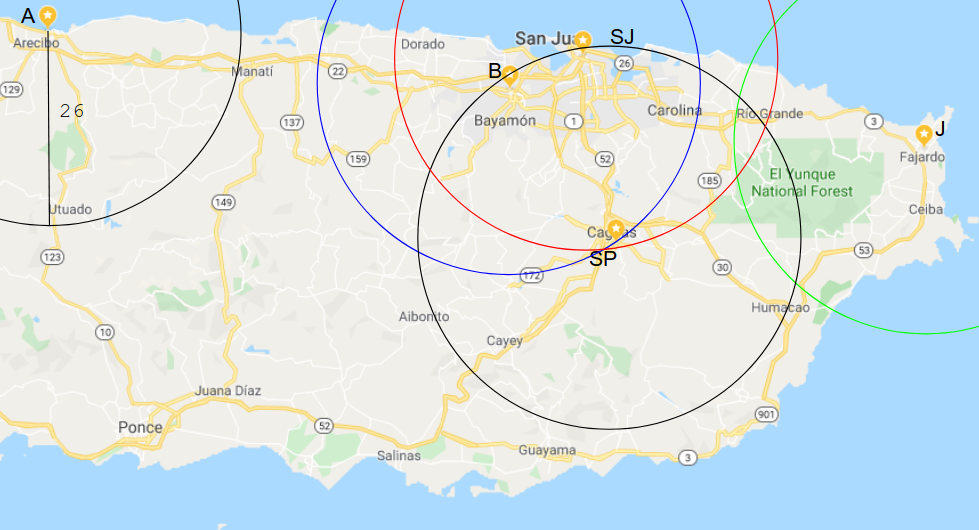
\includegraphics[width=0.75\textwidth]{hospital_radius_map.png}
    \caption{Map of Puerto Rico with 26 km Radii around Each Hospital}
    \label{fig:hospital_radius_map}
\end{figure}

We also can see from Figure \ref{fig:labeled_map} that Hospitals A, J are far away from the rest. So our choice of base locations is based on the two following concepts:
\begin{enumerate}
    \item All three containers must be used in order to serve all the hospitals
    \item At least one container must be within the flight radius of A and J
\end{enumerate}

By looking at Figure \ref{fig:hospital_radius_map} we see that the circle centered at Hospital A does not intersect with any of the other circles. This could lead us to believe that Hospital A will receive its own shipping container and base. However this is highly inefficient as Table \ref{tab:package_demand} shows that Hospital A only needs one MED 1 package per day. So it is important that we find a way to not designate an entire base just for Hospital A. 

One idea is to place a base location on the edge of the circle centered at Hospital A, and have Drone B fly within 52 km to another base and fully charge before delivering to another hospital. This would increase the output of each base and allow us to share cargo between bases. To demonstrate this idea, suppose we placed a base on the straight line path from A to B or from A to SP as shown in Figure \ref{fig:base_A_radius_map} by the red dot and blue dot, respectively, we see that if we have a base within a radii that equals to Drone B's maximum flight distance (52 km) then Drone B could reach these bases, charge, and deliver packages.

\begin{figure}[!ht]
    \centering
    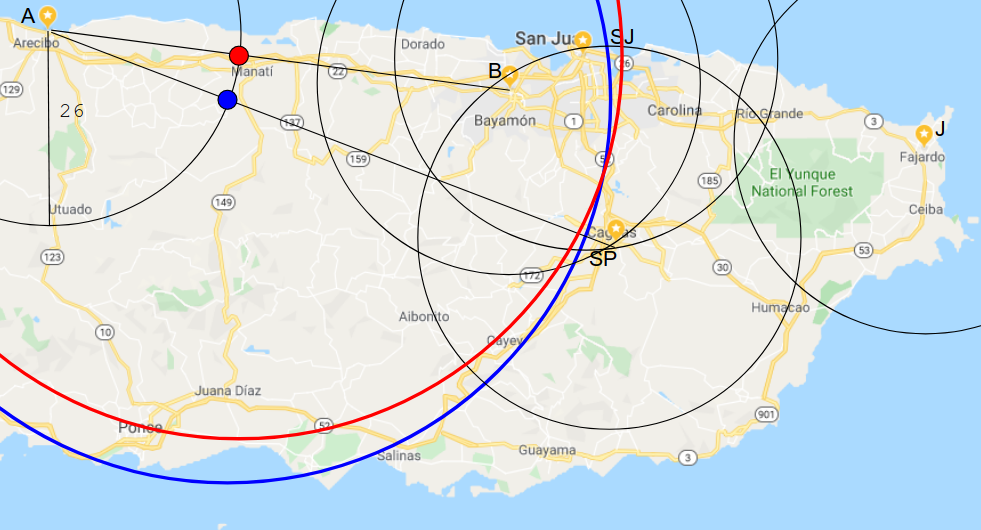
\includegraphics[width=0.75\textwidth]{base_A_radius_map.png}
    \caption{Map of Puerto Rico with 52km Radii around Potential Bases}
    \label{fig:base_A_radius_map}
\end{figure}

Now that we have determined it is possible to place the bases in a way which allows for drones to recharge during trips, we will choose three arbitrary base locations such that they are within 52 km of each at least one base. These arbitrary base locations are to demonstrate our intuition. In section 2.5, we explain a more detailed algorithm to show how we arrived at our final base locations. A potential base location formation is shown is Figure \ref{fig:theorhetical_bases}. Here we see that each base (the solid dots) is within 52 km of at least one other base, and all the hospitals are within 52 km of at least one base location. Furthermore, the black circles around each base represent the maximum distance that Drone B and reach and then return from in one trip, which is 26 km. This means that by using B Drones only, we are guaranteed to be able to service all the hospitals, since the drones can always fly to another base before departing for a hospital that is too far away to reach in one trip.

\begin{figure}[!ht]
    \centering
    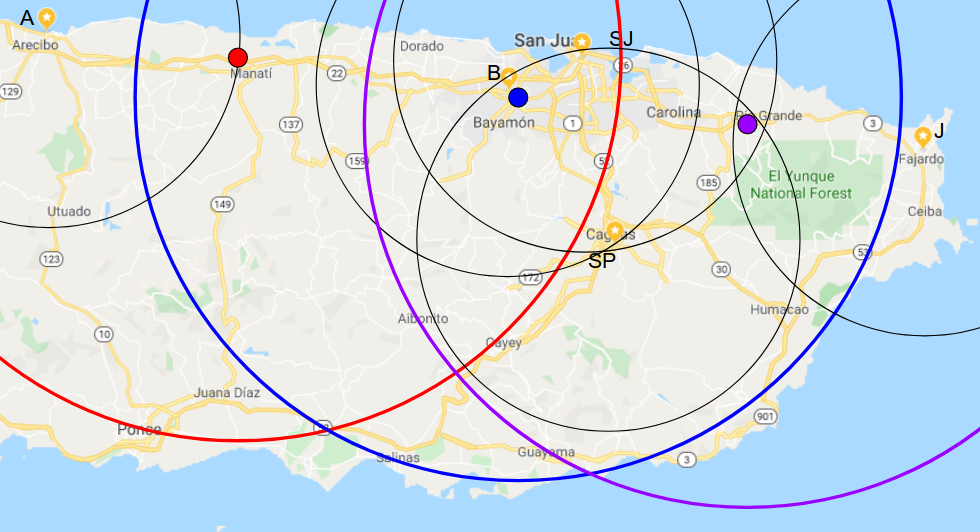
\includegraphics[width=0.75\textwidth]{theorhetical_bases.png}
    \caption{Map of Puerto Rico with Potential Base Locations that would allow us to service all the hospitals with only three B Drones}
    \label{fig:theorhetical_bases}
\end{figure}

Figure \ref{fig:base_graph_map} shows a more concise map with the potential base locations that we discussed above, as well as their theoretical respective distances from each other. Notice that stationing the base locations in such a way means that we could, in theory, service all the required hospitals with a single Drone B. However, we note that Drone B's cargo container holds less than other drones, which means we might not meet the daily medical package demand at all the hospitals. We will discuss how to actually choose these bases in the next section and provide an analytical explanation for our thinking.

\begin{figure}[!ht]
    \centering
    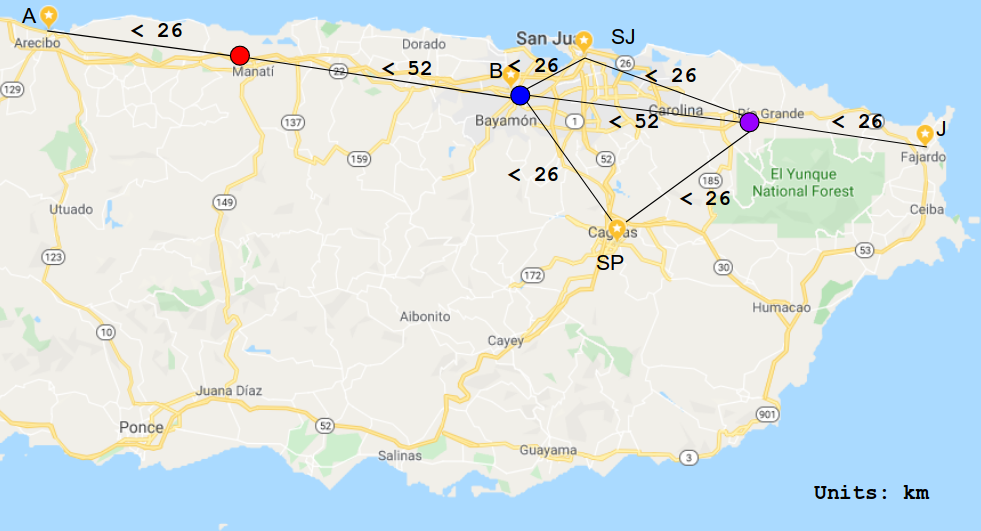
\includegraphics[width=0.75\textwidth]{base_graph_map.png}
    \caption{Map of Puerto Rico with Potential Base Locations and their theoretical respective distances from each other.}
    \label{fig:base_graph_map}
\end{figure}


\subsection{Developing the Model: Additional Assumptions}
\begin{table}[h]
    \centering
    \begin{tabular}{c|c}
    \hline Parameter & Description \\ 
    \hline $C_i$ & Container $i$ \\
    $D_i$ & Drone $i$ \\
    $r_d$ & Maximum flight range of Drone $d$ \\
    $H_i$ & Set of hospitals within flight radius of $C_i$ \\
    \end{tabular}
    \caption{Parameters}
    \label{tab:parameters}
\end{table}

\newenvironment{claim}[1]{\par\noindent\underline{Claim:}\space#1}{}
In the next few sections we develop a model that allows us to confirm our intuition above. We seek to find an optimal triple of locations for containers $C_1$, $C_2$, $C_3$ and the configuration of those containers. Recall we define "optimal" as the configuration that allows supplying the daily medicine requirements of all hospitals for the maximum number of days. We begin with the following assumptions:

\begin{itemize}
    \item Containers $C_1$, $C_2$, and $C_3$ contain single drones $D_1$, $D_2$, and $D_3$, respectively.
    \item All possible points of $C_1$, $C_2$, and $C_3$ are discretized to the nearest 0.05 degrees latitude/longitude.
    \item $C_1$ must be within 26.3 km of Hospital A, and $C_3$ must be within 26.3 km of Hospital J.
    \item $C_2$ cannot be within 26.3 km of Hospital A or Hospital J.
    \item All hospitals must be serviceable by at least one of $C_1$, $C_2$, and $C_3$.
    \item Resources can be shared freely between containers in the same group, where groups are as defined later in this section.
    \item The total number of days a group can serve its hospitals is the total volume of the group's selected drones subtracted from the total volume of the group's containers divided by the total volume of the group's daily required supplies.
    \item The number of days the island can be served is the minimum of the number of days each group can be served.
\end{itemize}
Justification of some of the less obvious assumptions follows.

\paragraph{Claim} All locations for $C_1$ must be within 26.35 km of Hospital A.
\begin{proof}
The above assumption is made necessary by our stated objective of serving all hospitals for as many days as possible. As we have assumed that drones cannot recharge outside of their base locations, this means that any drone that can reach a hospital must start from no more than half its maximum range away (so as to be able to make a round trip). As no drone has more than 52.67 km of maximum one-way range, any container that is further away than this from Hospital A cannot possibly reach its destination. We denote $C_1$ as the container that is chosen to satisfy this requirement.  
\end{proof}

\paragraph{Claim} All locations for $C_3$ must be within 26.35 km of Hospital J.
\begin{proof}
This claim follows similar logic as the previous claim pertaining to Hospital A. Any drone outside of this radius cannot possibly reach Hospital J and have enough range to return to its container base; therefore a container must be within this distance. We denote $C_3$ as the container that is chosen to satisfy this requirement.
\end{proof}

\paragraph{Claim} The remaining container, $C_2$, cannot be within the radii described by the above restrictions for $C_1$ and $C_3$.

\begin{figure}[!ht]
    \centering
    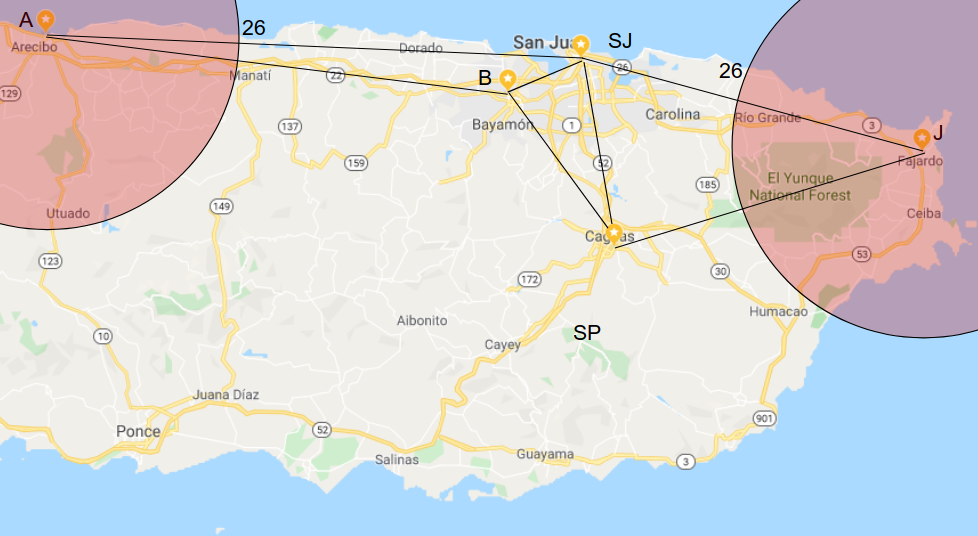
\includegraphics[width=0.75\textwidth]{2_4.png}
    \caption{An illustration showing proposed restrictions on locations of containers 1 and 3. Furthermore, container 2 cannot be within the depicted areas for containers 1 and 3.}
    \label{fig:2_4_map}
\end{figure}
\begin{proof}
The logic for this claim is not as immediately obvious as those of the prior two. \\
Observe in the Figure \ref{fig:labeled_map} that the distance from Hospital A to Hospital B is approximately 61 km. Any container that is within 26.35 km of Hospital A can therefore be no fewer than 34.65 km from Hospital B (this minimum occurs when the container sits directly on the line between Hospital A and Hospital B.) Therefore, a container within the specified radius cannot possibly serve Hospital B, as no drone has a flight radius exceeding 26.35 km. In such a case, $C_3$ also cannot reach Hospital B, as the minimum distance between Hospital J and Hospital B is 54.46 km - therefore, any container within 26.35 km of Hospital J is at least 28 km from Hospital B, so no drone starting from within this distance of Hospital J can serve Hospital B. \\
We have shown that any container within the required radius of Hospital A or within the required radius of Hospital J cannot serve Hospital B. In either case, this would violate our stated goal of serving all hospitals for as long as possible. We therefore conclude that the remaining container $C_2$ must not be within the radii required for $C_1$ and C3.
\end{proof}  

\newtheorem*{remark}{Remark}
\begin{remark}
Resources can be shared freely between containers in the same group. \end{remark}
We additionally propose that container locations can be grouped together if their locations are within the maximum flight range of each other's drones - for instance, if $C_1$ and $C_2$ are both using Drone B (with ~52 km maximum range) and are 40 km apart. Containers within a group can perform deliveries to hospitals within the flight radius of any of the containers within that same group by first stopping to recharge at another container within that group, so their volumes can be treated essentially as one larger container for the purposes of allocating supplies. We can define containers that are grouped together as the following:
\begin{align*}
    group(C_i) = group(C_j) \iff \Vert C_i - C_j \Vert \leq \frac{1}{2} r_{D_i} \text{ and } \Vert C_i - C_j \Vert \leq \frac{1}{2} r_{D_j} \\
    i, j \in {1, 2, 3}
\end{align*}
where $C_i$ and $C_j$ are two different containers, $D_i$ and $D_j$ are their corresponding drones, and $r_d$ is the maximum flight range of a drone $d$.

\subsection{Developing the Model: Constructing a Heuristic}
From these assumptions, we develop a way to approximate how many days we can supply all hospitals for, given a triple of container locations $(C_1, C_2, C_3)$ and their corresponding drone selections $(D_1, D_2, D_3)$:  

Let $H_i$ be the set of all hospitals that is within the "flight radius" of container $C_i$. That is,
\begin{align*}
    H_i = \{H: \Vert H - C_i \Vert \leq \frac{1}{2} r_{D_i}\}
\end{align*}
where $H$ is the location of one of the five hospitals, $C_i$ is a container, $D_i$ is the drone being used with that container, and $r_{D_i}$ is the maximum range of the drone $D_i$.   
Due to our assumption that all hospitals must be serviceable by at least one container, we have:
\begin{align*}
    \bigcup_i H_i = \{SJ, SP, F, A, B\}
\end{align*}
where $SJ$, $SP$, $F$, $A$, and $B$ are the hospitals for San Juan, San Pablo, Fajardo, Arecibo, and Bayamon, respectively.  We therefore can disregard any configuration of $C_i$ and $D_i$ for $i \in \{1, 2, 3\}$ for which this is not the case.
We group together the containers $C_1$, $C_2$, and $C_3$ to form between one and three groups $G_1$, $G_2$, $G_3$ using our earlier definition of groups:  
\begin{align*}
    i \in G_k \text{ and } j \in G_k \iff \Vert C_i - C_j \Vert \leq \frac{1}{2} r_{D_i} \text{ and } \Vert C_i - C_j \Vert \leq \frac{1}{2} r_{D_j} 
\end{align*}
We obtain sets $H_{G_k}$ for each group $G_k$ of the hospitals that the group can collectively reach, formed simply as the union of the $H_i$ of containers in the group:
\begin{align*}
    H_{G_k} = \bigcup_{i \in G_k} H_i
\end{align*}
Lastly, pooling together resources and container volume for all containers in each group, we can obtain the number of days each group can service its hospitals, and therefore the number of days for which we can serve all groups:
\begin{align*}
    &days (k) = \frac{\sum_{i \in G_k} (Volume (C_i) - Volume (D_i))}{Volume (M_k)/day} \\
    &days = \min_k (days (k))
\end{align*}
where $days (k)$ is the number of days for which Group $k$ can serve all its hospitals, and $days$ describes the number of days for which all Groups can be served. $M_k$ is the total amount of medical packages required by the hospitals in $H_{G_k}$.  We now must determine the configuration(s) $(C_1, C_2, C_3, D_1, D_2, D_3)$ of container locations and drone selections that maximize $days$.

\subsection{Developing the Model: Obtaining Solutions}
We iterate over all possible configurations $(C_1, C_2, C_3, D_1, D_2, D_3)$, for $C_1$,$C_2$, and $C_3$ as described in the above assumptions and $D_1$, $D_2$, $D_3$ are each one of drones B-G. (The R code used to perform these simulations is attached in the Appendix.)  

In Table \ref{tab:candidate_configs} is a selection of some of the candidate configurations that enable serving of all hospitals for the maximal 1146 days - the actual candidates are too numerous to list, as there are 6395 such potentially optimal configurations.

 \begin{table}[h]
    \centering
    \begin{tabular}{c|c|c|c|c|c||c}
    \hline Container 1 & Container 2 & Container 3 & Drone 1 & Drone 2 & Drone 3 & Max. Days \\
    \hline
    (18.4, -66.5) & (18.3,-66.1) & (18.1,-65.7) & B & B & B & 1146 \\
    (18.3, -66.6) & (18.3,-66.2) & (18.2,-65.8) & B & B & B & 1146 \\
    (18.25, -66.65) & (18.25,-66.2) & (18.2,-65.85) & B & B & B & 1146 \\
    \end{tabular}
    \caption{Some candidate configurations for optimal placement/drone selections}
    \label{tab:candidate_configs}
\end{table}
We acquire through these simulations a set of configurations, each consisting of locations for containers $C_1$, $C_2$, and $C_3$, as well as their corresponding choices of drones $D_1$, $D_2$, and $D_3$. These stored configurations are such that they allow for supplying of all hospitals for the maximal number of days. In these configurations, we observe all three containers are grouped together, as $C_2$ is within maximum flight range of both $C_1$ and $C_3$. Therefore, we can freely allocate medical supplies between all three containers. In all three containers Drone B is selected for use, likely a consequence of its comparatively longer range and smaller required volume. These maximally efficient allocations allow us to supply all hospitals for up to 1146 days.   

We see that if we consider ranges of the simulation with 0.05 granularity, we get approximately the following potential optimal base locations: 
\begin{table}[h]
    \centering
    \begin{tabular}{c|c|c|c|c}
        \hline
        Base &  Min. Latitude & Max. Latitude & Min. Longitude & Max. Longitude \\
        \hline 1 & 18.25 & 18.45 & -66.65 & -66.45 \\
        2 & 18.25 & 18.45 & -66.15 & -66.1 \\
        3 & 18.1 & 18.4 & -65.85 & -65.65 \\
    \end{tabular}
    \caption{Possible Base locations given by the simulation}
    \label{tab:candidate_ranges}
\end{table}

\begin{figure}[h]
    \centering
    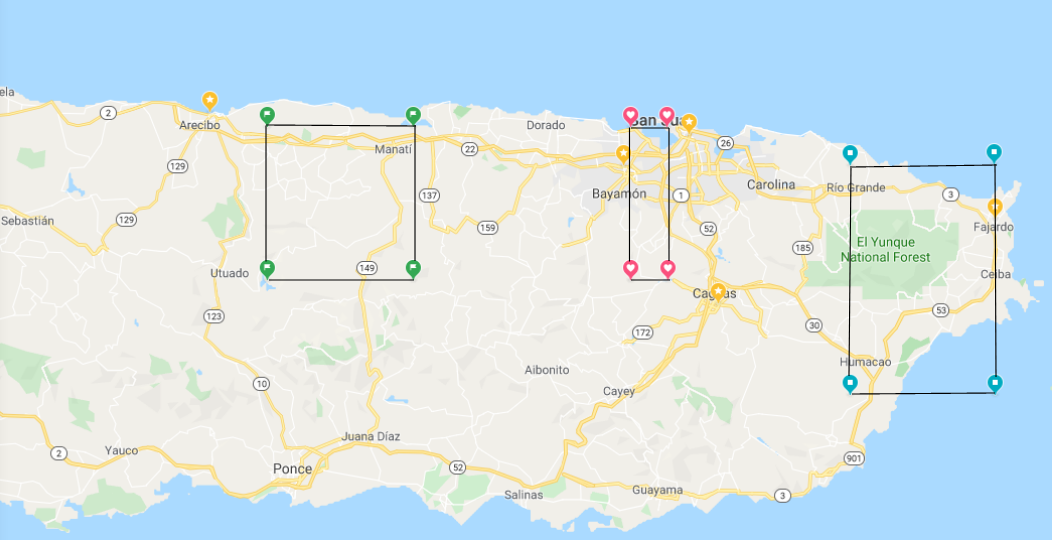
\includegraphics[width=0.75\textwidth]{2_3.png}
    \caption{Approximate potential base locations after initial simulations}
    \label{fig:2_3_map}
\end{figure}

It remains to optimize within the set of our acquired "candidate locations" for the maximum possible amount of road reconnaissance. This refinement of our solution set is considered in the section below.

\subsection{Refinement for Road Reconnaissance}

From the above simulation we end up with a set of triples of candidate locations for our shipping containers. All of these locations allow us to group together all three containers as one (due to being within one-way flight range of each other's drones), and allow us to supply all hospitals on the island for a maximum of 1146 days. Furthermore, we note that all such configurations have all three containers use Drone B.   

Of particular importance is that the combination of 1146 days' worth of medical supplies and three 'B' drones consumes nearly all of the three containers' volumes; indeed, in each such configuration we only have 4260 in$^3$ of space remaining:
\begin{align*}
   (\sum_i (Volume (C_i) - Volume (D_i)) - 1146 * Volume(M_i)/day) = 4260
\end{align*}
where, as before, $C_i$ and $D_i$ are the containers and their corresponding drones, and $M_i$ is the volume of daily required medical supplies for hospitals within range of $C_i$.  

While more medical supplies can be fit in such a volume, no drone has a volume of fewer than 12500 in$^3$ - therefore, we cannot use additional drones to monitor the state of Puerto Rico's roads. As we have assumed that supplying Puerto Rico's hospitals is paramount, we therefore do not consider removing supplies to fit additional drones, and instead optimize within the constraints of the "optimal" configurations acquired above.  

To perform this optimization, we require several additional assumptions:
\begin{itemize}
\item We can again discretize Puerto Rico's geography into a grid of points a fixed distance (in latitude/longitude coordinates) apart. Each point can be assumed to be at the center of a grid square representing the surrounding area.
\item We limit consideration of roads to major (numbered) highways.
\item Each square (as represented by the point at its center) can be thought of as having roads in it or not having roads in it. All squares containing roads are assumed to have an equal length of road within.
\item Given our grid system of points, we can manually exclude those representing areas that have no road (e.g. over water, or in mountainous or forested terrain). 
\item Not all roads need to be monitored every day; road recon can be done over an indefinite period of time.
\end{itemize}  

We therefore define the optimal placement for our three containers as the one that has the most of these road grid points within the flight radius of its drones. We further note that this will always be the range of Drone B, as all containers contain one Drone B and, when filled with medical supplies, cannot hold additional drones.  

For each set of points and their drones, we consider the amount of roads that can be surveyed to be represented by the number of "road points" described above that are within the flight radius of Drone B from all of the three containers. (Recall that in our candidate configurations, all containers use Drone B.) The configuration with the largest number of such points that is within the flight radii is therefore the "best" configuration.  We begin by laying a grid of points over Puerto Rico that are 0.05 latitude/longitude degrees apart, as in the earlier simulation. We proceed to manually remove from this grid all points that are considered to not have any major highways in their corresponding regions, such as in forests or over water. We end up with a set of "road points" representing sectors of this grid that contain major highways. The map of these road points is depicted below in Figure \ref{fig:roadpoints_map}.

\begin{figure}[h]
    \centering
    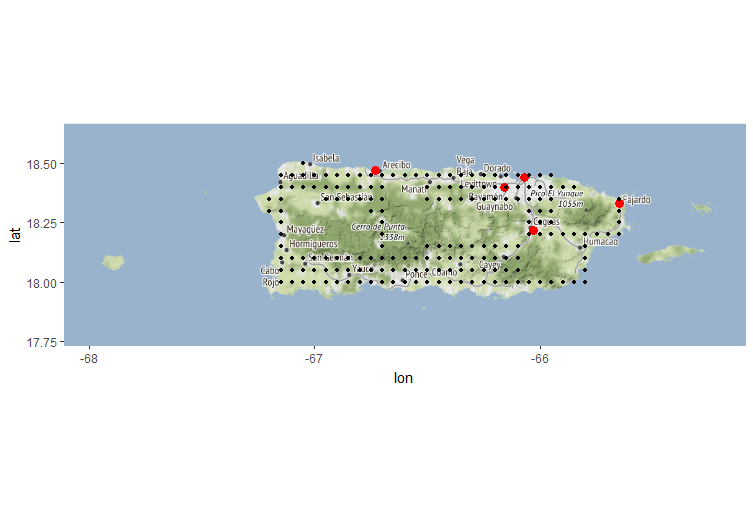
\includegraphics[width=0.75\textwidth]{roadpoints.png}
    \caption{A map of points representing areas with major highways.}
    \label{fig:roadpoints_map}
\end{figure}

We take these points and convert them to kilometer distances using the same conversion as before: we assume that one degree latitude corresponds to 110.68 km, and that one degree longitude corresponds to 105.71 km. For every candidate configuration acquired earlier, we use simple distance calculations to count the total number of road points that are within flight radius of at least one container:
\begin{align*}
    roadpoints(c_1, c_2, c_3) &= \sum_{i=1}^{3} r(c_i) \\
    r(c) &= \sum_{x \in R} reachable(c, x) \\
    reachable(c, x) &= 
    \begin{cases}
        1 & \Vert c -x\Vert < 0.5 * r_b \\
        0 & otherwise
    \end{cases} \\
\end {align*}
Where $c_1$, $c_2$, $c_3$ are the locations of containers 1, 2, and 3, $R$ is the set of "road points" as illustrated in Figure \ref{fig:roadpoints_map}, and $r_b$ is the maximum flight range of Drone B. (Recall that all candidate configurations use Drone B in all cases.)  

Once again we iterate over all possible configurations, this time using only the configurations that were candidates for optimal configuration as found in the prior simulation. For each configuration, we simply sum the number of road points that are within one-half the maximum range of Drone B, as all such configurations exclusively use Drone B. 
After performing the simulation on all candidate configurations, we find that there exists a unique best configuration:
\begin{table}[h]
    \centering
    \begin{tabular}{c|c|c||c|c}
    \hline Container 1 & Container 2 & Container 3 & Days  & Reachable road points\\
    \hline
    (18.25, -66.65) & (18.25,-66.2) & (18.2,-65.85) & 1146 & 97\\
    \end{tabular}
    \caption{The unique optimal configuration}
    \label{tab:best_config}
\end{table}

\begin{figure}[h]
    \centering
    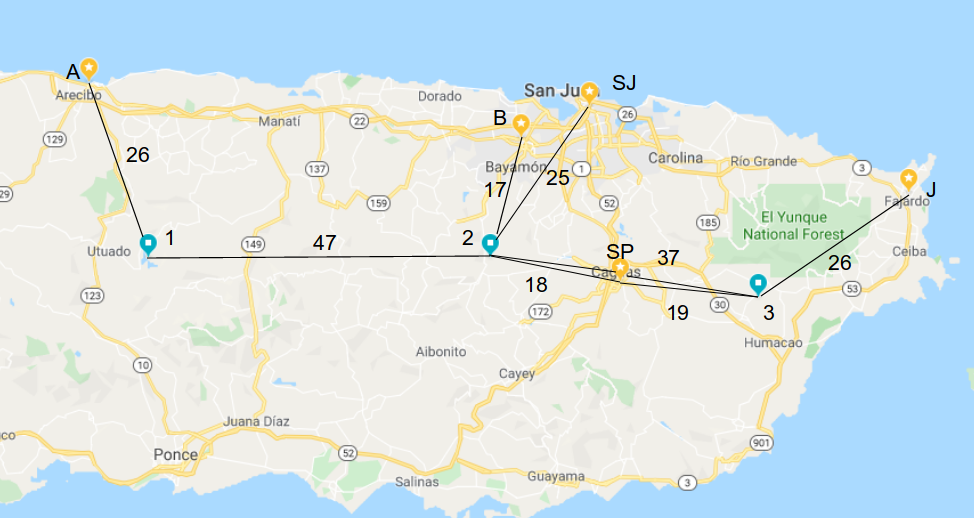
\includegraphics[width=0.75\textwidth]{2_5.png}
    \caption{Our optimal base locations based on optimizing for road surveillance}
    \label{fig:2_5_map}
\end{figure}

Under our assumptions, of the configurations that were considered by our simulations, this is a configuration that maximizes the number of days for which we can fulfill the daily needs of all hospitals, and within those configurations uniquely maximizes the amount of roads that can be monitored. We therefore recommend that HELP, Inc. use containers at 18.25 N 66.65 W, 18.25 N 66.2 W, and 18.2 N 65.85 W, each containing a single Drone B.   

Under our assumptions, the above configuration is the best if it is viable - that is, that it is possible for all the hospitals to have their daily requirements fulfilled while leaving time for road reconnaissance to be performed. It remains to be shown that this configuration is in fact viable, and to develop a flight plan and schedule that implements it.  

\subsection{Cargo Arrangement}

Since we chose our bases based on drone B, our cargo arrangement will be based on using drone B. In order to maximize the space in the container used for packages, we will have one drone B per container only. We will later show that having one drone B is enough to deliver all the packages to the hospitals and still have some time for road surveillance. 

We assumed that all the hospitals daily needs are of the same importance, so we will start by dividing the available volume of all three containers by the daily volume for all the packages needed by the hospitals. We do this to ensure that all hospitals are serviced for the same number of days. Note that this computation was made during our iterations under constructing a model, but just to reiterate and show our reasoning, we wanted to show how we came to the number of days shown above by hand, which will help us figure out the cargo arrangement. 

Table \ref{tab:tot_daily_vol} will be useful for our calculations. This table uses information from tables \ref{tab:package_demand} and \ref{tab:med_config}.
\begin{table}[h]
    \centering
    \begin{tabular}{c|c|c}
    \hline Hospital Location &  Volume of all Packages Per Day (in$^3$/Day) & Weight (lb/Day) \\
    \hline
    J (Fajardo) & 826 & 5\\
    SP (San Pablo) & 1316 & 7\\
    SJ (San Juan) &  690 & 4\\
    B (Bayamon) & 1852 & 12\\
    A (Arecibo) & 490 & 2\\
    \hline
    Total &  5174 & 30\\
    \hline
    
    \end{tabular}
    \caption{Total Volume Per Day and Weight Per Day}
    \label{tab:tot_daily_vol}
\end{table}


\begin{equation}
    \text{Volume of Drone B} = 30 \times 30 \times 22 = 19,800 in^3
    \label{eq:B_vol}
\end{equation}

From table \ref{tab:cargo_container_config}, we know, that the volume of the single cargo container is 1,997,688 in$^3$. So: 

\begin{equation}
    \text{Available Volume for MED for all Containers} = 3 \times 1,997,688 - 3 \times 19,800 = 5,933,664 \: \text{in$^3$}
    \label{eq:avail_vol_all}
\end{equation}
\begin{equation}
    \text{Available Volume for MED in single container} = \frac{5,933,664}{3} = 1,977,888 \: \text{in$^3$}
    \label{eq:avail_vol}
\end{equation}
\begin{equation}
    \text{Number of Days} = \frac{5,933,664}{5174} = 1146.823348 \approx 1146 \: \text{Days}
    \label{eq:B_vol}
\end{equation}

Now that we know the number of days, we can figure out the number of overall volume that must be stored in the cargo containers for each of the hospitals (for all 1146 Days). We do this by multiplying the volume/day in table \ref{tab:tot_daily_vol} for each of the hospitals by 1146. This gives us the results shown below:

\begin{table}[h]
    \centering
    \begin{tabular}{c|c}
    \hline Hospital Location & Volume of all Packages (in$^3$) \\
    \hline
    J (Jajardo) & 946,596\\
    SP (San Pablo) & 1,508,136\\
    SJ (San Juan) & 790,740\\
    B (Bayamon) & 2,122,392\\
    A (Arecibo) & 561,540\\
    \hline
    Total & 5,929,404\\
    \hline
    \end{tabular}
    \caption{Total Volume for Total Days}
    \label{tab:tot_vol}
\end{table}

The idea is that we store as much daily packages/volume as we can in the closest container to the hospital. Note that depending on which container we start organizing for, the arrangement will differ slightly. In hope of  maximizing efficiency, we will start arrangements from the hospital that requires the greatest space (volume) in our containers to the hospital that requires the least space (volume). We do this because we reason that the hospital that requires the greatest volume would require the most trips by drone B to fulfill its needs. Since we aim to minimize the time it takes for our drones to deliver all the packages, we want to minimize the total distance traveled by the drones. One way to do that is by minimizing the distance traveled by the drone that has to travel the most trips. A helpful table is table \ref{tab:tot_vol} the one below, which shows the distance of each of the hospitals to each of the containers as well as the distance of the containers to one another. To calculate this distance, we used an online calculator that measures the distance between longitude/latitude locations \cite{dist_calc}.



We start by looking at hospital B, which we know needs the most storage space for its packages. From table \ref{tab:tot_vol}, we know that hospital B needs 2,122,392 in$^3$ in volume, which is greater than the volume of a single container, so we will store as much as we can in the closest container then the leftover will go to the second closest container. From figure \ref{fig:2_5_map}, the closest container to B is container 2, and the second closest container is container 3. We can do this by: 

\begin{itemize}
\item Store 1067 days-worth of packages in container 2\\
\\Days stored in Container 2=Available Volume/Daily Volume of B=$\frac{1,977,888}{1852}$=1067 Days \\
This corresponds to 2134 MED 1 packages, 1067 MED 2 packages, and 2134 MED 3 packages. 
\item The remaining 79 days worth of packages will be stored in container 3\\
Remaining Days=1146-1067=79 Days\\
This corresponds to 158 MED 1 packages, 79 MED 2 packages, and 158 MED 3 packages. 
\end{itemize}

Looking at hospital SP in table \ref{tab:tot_vol}, we know that it needs 1,508,136in$^$ of space. From figure \ref{fig:2_5_map}, we know the closest container to SP is container 2, but container 2 is essentially full. The second closest container is container 3, which is not completely full but not completely empty. 

\begin{itemize}
\item Looking at the remaining space in container 3, we can tell that it fits all of SP's packages. 
Remaining Volume in Container 3 = 1,977,888-79$\times$1852 = 1,831,580 in$^3$\\
So in container 3, we now also have 2292 MED 1 packages and 1146 MED 3 packages. 
\end{itemize}

Looking at hospital J in table \ref{tab:tot_vol}, we know it needs 946,596in$^3$ of space. From figure \ref{fig:2_5_map}, We can tell that the closest container to container 3, which is not full but not empty, then container 2, which is full, then container 1:

\begin{itemize}
\item We look at how much space we have left in container 3, and try to fill it\\
Remaining Volume in Container 3 = 1,831,580 -1,508,136=323,444 in$^3$
\item This remaining volume can hold 390 days-worth of packages\\
Days stored in Container 3=Available Volume/Daily Volume of J=$\frac{323,444}{826}$=391 Days \\
This corresponds to 391 MED 1 packages and 391 MED 3 packages. 
\item The remaining 755 days worth of packages will be stored in container 1\\
Remaining Days=1146-390=755 Days\\
This corresponds to 755 MED 1 packages and 755 MED 3 packages. 
\end{itemize}

Now that containers 2 and 3 are full, we know that the packages for the remaining two hospitals must be stored in container 1. But, to check that we didn't make any errors, we will make some calculations. 
\begin{itemize}
\item The remaining volume in container 1 is \\
Remaining volume in Container 1= 1,977,888-755$\times$826=1,354,258 in$^3$
\item This remaining volume clearly fits all the packages for hospitals SJ and A\\
Volume for Hospital SJ and A= 790,740+561,540=1,352,280 in$^3$.\\
This volume is clearly less than the volume we have i.e. the packages fit. \\
So, container 1 also has 2292 MED 1 packages (1146 for hospital SJ and 1146 for hospital A) and 1146 MED 2 packages (for hospital SJ). 
\end{itemize}

We now know where the packages for each of the hospitals are located, which will guide us in making the daily schedule for the drones. Before doing that, let's summarize the hospitals that each of the containers will service: 

\begin{itemize}
    \item Container 1: For the first 391 days, container 1 service hospitals A and SJ. For the last 755 days, container 1 service hospitals A, SJ, and J. 
    \item Container 2: For the entire 1146 days, container 2 services hospital B only. 
    \item Container 3: For the first 391 days, container 3 services hospitals SP and J. For the last 79 days, container 3 services hospitals SP and B. And for the remaining 676 days in-between days, container 3 only services hospital SP. 
\end{itemize}

\subsection{Flight Plan and Scheduling}

Note that the below flight paths and times are for pre-surveillance. Recall, that we take charging time for drone B to be 1.5 hours. \\

Container 1:\\
Note that weight and volume of packages for hospitals A, SJ, and J (individually) fit the volume and weight conditions for drone B. This can be checked by referring to tables \ref{tab:tot_daily_vol}, \ref{tab:drones_info}, and \ref{tab:cargo_bay_config}. \\
\begin{itemize}
    \item First 391 days: Flight path is from container 1 to A and back, then drone charges, then from container 1 to 2, then drone charges, then from container 2 to SJ and back, then drone charges, and finally from 2 to 1.\\ 
    \\
    Time Taken= $\frac{26 \times 2}{79}$ + 1.5 + $\frac{47}{79}$ + 1.5 $\frac{26 \times 2}{79}$ +1.5 +  $\frac{47}{79}$ $\approx$ 7.00 hours
    \item Last 755 day:, the drone follows the same above flight, then charges, then goes from container 1 to 2, then drone charges, then from container 2 to 3, then drone charges, then from container 3 to J and back, then drone charges, then from container 3 to 2, then charges, then from container 2 to 1. \\
    \\
     Time Taken= 7.00+$\frac{47}{79}$ + 1.5 + $\frac{37}{79}$ + 1.5 $\frac{26 \times 2}{79}$ +1.5 +  $\frac{37}{79}$ + 1.5 + $\frac{47}{79}$  $\approx$ 7.00 + 1.5 + 8.78 $\approx$ 15.78 hours
    
    
\end{itemize}

Container 2:\\
Note that the weight and volume of packages for hospital B exceed drone B's restriction. So, we will have to send the materials in two trips. The first trip delivers 2 MED 1 packages and the second trip delivers 1 MED 2 and 2 MED 3 packages).\\  
\begin{itemize}
    \item For all : Flight path is from container 2 to B and back, then drone charges, then from container 2 to B and back.\\ 
    \\
    Time Taken= $\frac{17 \times 2}{79}$ + 1.5 + $\frac{17 \times 2}{79}$ $\approx$ 2.36 hours
\end{itemize}

Container 3:\\
Note that weight and volume of packages for hospitals SP exceeds drone B's restrictions. So, we will have to send the materials in two trips. The first trip delivers 1 MED 1 and 1 MED 3 packages and the second trip delivers 1 MED 1 package). Hospital B also needs two trips as described above under container 2. Hospital J fits all its packages in one trip.\\

\begin{itemize}
    \item 676 days in-between: Flight path is from container 3 to SP and back, then drone charges, then from container 3 to SP and back.\\ 
    Time Taken= $\frac{19 \times 2}{79}$ + 1.5 + $\frac{19 \times 2}{79}$ $\approx$ 2.46 hours
    \item First 391 days: The drone follows the same flight above (as the 676 days) then charges, then from container 3 to J and back. 
    \\
    Time Taken= 2.46 + 1.5 + $\frac{26 \times 2}{79}$ $\approx$ 4.62 hours
    \item Last 79 days: At this point drone B in container 2 would no longer be used for hospital deliveries from container 2, so after it finishes its duties for its last delivery day and conducts appropriate surveillance, it can be sent to container 3 to be charged and used the next day. So, we have two available drones at container 2 now. One of them follows the exact path of drone B outlines in the 676 days in-between. The other one goes from container 3 to container 2 then charges, then from container 2 to hospital B and back, then charges, then from container 3 to 2, then charges and repeat the process once more. \\
    \\
     Time Taken= 2 $\times$ ($\frac{19+18}{79}$ + 1.5 + $\frac{26 \times 2}{79}$ + 1.5 + $\frac{19+18}{79}$)+1.5 $\approx$ 6.09 hours
    
    
\end{itemize}

We suggest that deliveries for hospitals be made around 6 hours before sunset. So, we get 6 hours of deliveries made in daylight, and the rest of the deliveries can be made at night. This also gives us at least 6 hours for surveillance. 


















 





